\documentclass{beamer}
\mode<presentation>
\usepackage{amsmath}
\usepackage{amssymb}
%\usepackage{advdate}
\usepackage{adjustbox}
\usepackage{subcaption}
\usepackage{enumitem}
\usepackage{multicol}
\usepackage{mathtools}
\usepackage{listings}
\usepackage{url}
\usepackage{hyperref}
\def\UrlBreaks{\do\/\do-}
\usetheme{Boadilla}
\usecolortheme{lily}
\setbeamertemplate{footline}
{
  \leavevmode%
  \hbox{%
  \begin{beamercolorbox}[wd=\paperwidth,ht=2.25ex,dp=1ex,right]{author in head/foot}%
    \insertframenumber{} / \inserttotalframenumber\hspace*{2ex} 
  \end{beamercolorbox}}%
  \vskip0pt%
}
\setbeamertemplate{navigation symbols}{}

\providecommand{\nCr}[2]{\,^{#1}C_{#2}} % nCr
\providecommand{\nPr}[2]{\,^{#1}P_{#2}} % nPr
\providecommand{\mbf}{\mathbf}
\providecommand{\pr}[1]{\ensuremath{\Pr\left(#1\right)}}
\providecommand{\qfunc}[1]{\ensuremath{Q\left(#1\right)}}
\providecommand{\sbrak}[1]{\ensuremath{{}\left[#1\right]}}
\providecommand{\lsbrak}[1]{\ensuremath{{}\left[#1\right.}}
\providecommand{\rsbrak}[1]{\ensuremath{{}\left.#1\right]}}
\providecommand{\brak}[1]{\ensuremath{\left(#1\right)}}
\providecommand{\lbrak}[1]{\ensuremath{\left(#1\right.}}
\providecommand{\rbrak}[1]{\ensuremath{\left.#1\right)}}
\providecommand{\cbrak}[1]{\ensuremath{\left\{#1\right\}}}
\providecommand{\lcbrak}[1]{\ensuremath{\left\{#1\right.}}
\providecommand{\rcbrak}[1]{\ensuremath{\left.#1\right\}}}
\theoremstyle{remark}
\newtheorem{rem}{Remark}
\newcommand{\sgn}{\mathop{\mathrm{sgn}}}
\providecommand{\abs}[1]{\left\vert#1\right\vert}
\providecommand{\res}[1]{\Res\displaylimits_{#1}} 
\providecommand{\norm}[1]{\lVert#1\rVert}
\providecommand{\mtx}[1]{\mathbf{#1}}
\providecommand{\mean}[1]{E\left[ #1 \right]}
\providecommand{\fourier}{\overset{\mathcal{F}}{ \rightleftharpoons}}
%\providecommand{\hilbert}{\overset{\mathcal{H}}{ \rightleftharpoons}}
\providecommand{\system}{\overset{\mathcal{H}}{ \longleftrightarrow}}
	%\newcommand{\solution}[2]{\textbf{Solution:}{#1}}
%\newcommand{\solution}{\noindent \textbf{Solution: }}
\providecommand{\dec}[2]{\ensuremath{\overset{#1}{\underset{#2}{\gtrless}}}}
\newcommand{\myvec}[1]{\ensuremath{\begin{pmatrix}#1\end{pmatrix}}}
\let\vec\mathbf

\lstset{
%language=C,
frame=single, 
breaklines=true,
columns=fullflexible
}

\numberwithin{equation}{section}

\title{NCERT-10.4.1.2.2}
\author{Arnav Mahishi \\ Dept. of Electrical Engg.\\IIT Hyderabad.}

\date{\today} 
\begin{document}

\begin{frame}
\titlepage
\end{frame}
\section*{Outline}
\section{Problem}
\begin{frame}
\frametitle{Problem Statement}
Find out whether the lines $5x-4y+8=0$ and $7x+6y-9=0$ intersect at a point, parallel or coincident 
\end{frame}
%\subsection{Literature}
\section{Solution}
\subsection{Input Parameters}
\begin{frame}
\frametitle{Input Parameters}
\begin{table}[h!]
    \centering
    \begin{tabular}[12pt]{ |c| c|}
    \hline
    \textbf{Variable} & \textbf{Description}\\ 
    \hline
     $A$& Matrix consisting of coefficients in the linear equation\\
     \hline
     $L$& Lower triangular matrix\\
     \hline
     $U$& Upper triangular matrix\\
     \hline
     $\vec{x}$ & Solution to the linear equation\\
     \hline
    \end{tabular}
    \label{tab:my_label}
\end{table}
\end{frame}
\subsection{Theoritical Soln}
\begin{frame}
\frametitle{Theoritical Soln}
Let $a_1$,$b_1$, and $c_1$ and $a_2$,$b_2$, and $c_2$ be the coefficents of $x$,$y$, and $1$ in lines $1$ and $2$ respectively.\\
We get:
\begin{align}
    \frac{a_1}{a_2}=\frac{5}{7}\\
    \frac{b_1}{b_2}=\frac{-2}{3}\\
    \frac{c_1}{c_2}=\frac{-8}{9}\\
    m_1=\frac{-a_1}{b_1}=\frac{5}{4}\\
    m_2=\frac{-a_2}{b_2}=\frac{7}{6}
\end{align}
As all the ratios aren't equal to each other neither are $m_1$ and $m_2$ equal\\
$\therefore$ The lines intersect at a point\\
\end{frame}
\subsection{Computational Soln}
\begin{frame}
    \frametitle{Computational Soln}
    \textbf{Computational Solution:}\\
The set of linear equations $5x-4y+8=0$ and $7x+6y-9=0$ can be represented by the following equation
\begin{align}
    \myvec{5&-4\\7&6}\myvec{x\\y}=\myvec{-8\\9}
\end{align}
Any on-singular matrix can be represented as a product of a lower triangular matrix $L$ and an
upper triangular matrix $U$:
\begin{align}
    A = L \cdot U
\end{align}
1. Initialization: 
   - Start by initializing $ \mathbf{L} $ as the identity matrix $ \mathbf{L} = \mathbf{I} $ and $ \mathbf{U} $ as a copy of $ \mathbf{A} $.
   
2. Iterative Update:
   - For each pivot $ k = 1, 2, \ldots, n $:
     - Compute the entries of $ U $ using the first update equation.
     - Compute the entries of $ L $ using the second update equation.

3. Result:
   - After completing the iterations, the matrix $ \mathbf{A} $ is decomposed into $ \mathbf{L} \cdot \mathbf{U} $, where $ \mathbf{L} $ is a lower triangular matrix with ones on the diagonal, and $ \mathbf{U} $ is an upper triangular matrix.
\end{frame}
\begin{frame}
\subsection*{1. Update for $ U_{k,j} $ (Entries of $ U $)}

For each column $ j \geq k $, the entries of $ U $ in the $ k $-th row are updated as:
\[
U_{k,j} = A_{k,j} - \sum_{m=1}^{k-1} L_{k,m} \cdot U_{m,j}, \quad \text{for } j \geq k.
\]
This equation computes the elements of the upper triangular matrix $ \mathbf{U} $ by eliminating the lower triangular portion of the matrix.

\subsection*{2. Update for $ L_{i,k} $ (Entries of $ L $)}

For each row $ i > k $, the entries of $ L $ in the $ k $-th column are updated as:
\[
L_{i,k} = \frac{1}{U_{k,k}} \left( A_{i,k} - \sum_{m=1}^{k-1} L_{i,m} \cdot U_{m,k} \right), \quad \text{for } i > k.
\]
This equation computes the elements of the lower triangular matrix $ \mathbf{L} $, where each entry in the column is determined by the values in the rows above it.\\
Using a code we get L,U as 
\end{frame}
\begin{frame}
\textbf{Step-by-Step Process:}\\

\textbf{1. Initial Matrix:}
\begin{align}
    A = \myvec{5 & -4 \\ 7 & 6}
\end{align}

\textbf{2. Compute $U$ (Upper Triangular Matrix):}\\
Using the update equation for $U$:
\begin{align}
    U_{11} = A_{11} = 5, \quad U_{12} = A_{12} = -4
\end{align}
For $U_{22}$:
\begin{align}
    U_{22} = A_{22} - L_{21} \cdot U_{12} = 6 - \frac{7}{5} \cdot (-4) = \frac{58}{5}
\end{align}

\textbf{3. Compute $L$ (Lower Triangular Matrix):}\\
Using the update equation for $L$:
\begin{align}
    L_{21} = \frac{A_{21}}{U_{11}} = \frac{7}{5}
\end{align}
The final $L$ matrix is:
\begin{align}
    L = \myvec{1 & 0 \\ \frac{7}{5} & 1}
\end{align}
\end{frame}
\begin{frame}
\textbf{4. Solving the System:}\\
Using the equations $L\vec{y} = \vec{b}$ and $U\vec{x} = \vec{y}$:
\begin{itemize}
    \item \textbf{Forward Substitution:}
    \begin{align}
        \myvec{1 & 0 \\ \frac{7}{5} & 1}\myvec{y_1 \\ y_2} = \myvec{-8 \\ 9}
    \end{align}
    Solving gives:
    \begin{align}
        y_1 = -8, \quad y_2 = \frac{101}{5}
    \end{align}

    \item \textbf{Backward Substitution:}
    \begin{align}
        \myvec{5 & -4 \\ 0 & \frac{58}{5}}\myvec{x_1 \\ x_2} = \myvec{-8 \\ \frac{101}{5}}
    \end{align}
    Solving gives:
    \begin{align}
        x_2 = \frac{101}{58}, \quad x_1 = \frac{-6}{29}
    \end{align}
\end{itemize}

Thus, the solution is:
\begin{align}
    \vec{x} = \myvec{\frac{-6}{29} \\ \frac{101}{58}}
\end{align}
\end{frame}
\begin{frame}{Plot}
\begin{figure}[h!]
   \centering
   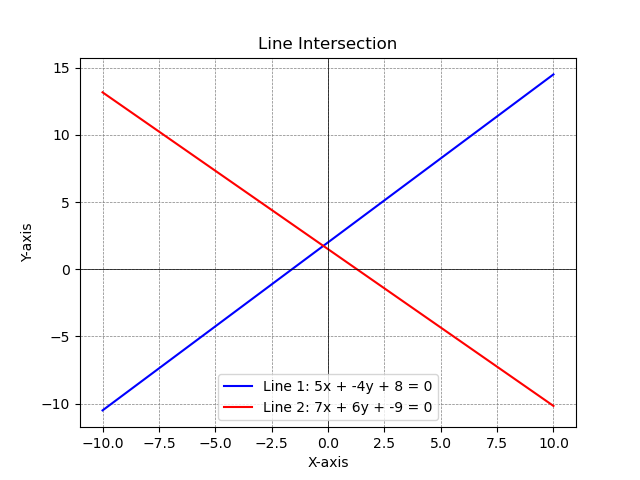
\includegraphics[width=0.7\columnwidth]{../../assignments/Problem 6/figs/fig.png}
    \caption{Solution to set of linear equations}
\end{figure}
\end{frame}
\end{document}
